
\chapter{Total boundness of reloids}


\section{Thick binary relations}
\begin{defn}
\index{alpha-thick@$\alpha$-thick}I will call \emph{$\alpha$-thick} and denote $\thick_{\alpha}(E)$
a $\mathbf{Rel}$-endomorphism $E$ when there exists a finite cover $S$
of $\Ob E$ such that $\forall A\in S:A\times A\subseteq\GR E$.
\end{defn}

\begin{defn}
$\CS(S)=\bigcup\setcond{A\times A}{A\in S}$ for a collection $S$
of sets.\end{defn}
\begin{rem}
$\CS$ means ``Cartesian squares''.\end{rem}
\begin{obvious}
A $\mathbf{Rel}$-endomorphism is $\alpha$-thick iff there exists
a finite cover $S$ of $\Ob E$ such that $\CS(S)\subseteq\GR E$.\end{obvious}
\begin{defn}
\index{beta
-thick@$\beta$-thick}I will call \emph{$\beta$-thick} and denote $\thick_{\beta}(E)$
a $\mathbf{Rel}$-endomorphism $E$ when there exists a finite set
$B$ such that $\rsupfun{\GR E}B=\Ob E$.\end{defn}
\begin{prop}
$\thick_{\alpha}(E)\Rightarrow\thick_{\beta}(E)$.\end{prop}
\begin{proof}
Let $\thick_{\alpha}(E)$. Then there exists a finite cover $S$ of
the set $\Ob E$ such that $\forall A\in S:A\times A\subseteq\GR E$.
Without loss of generality assume $A\ne\emptyset$ for every $A\in S$.
So $A\subseteq\rsupfun{\GR E}\{x_{A}\}$ for some $x_{A}$ for every
$A\in S$. So
\[
\rsupfun{\GR E}\setcond{x_{A}}{A\in S}=\bigcup\setcond{\rsupfun{\GR E}\{x_{A}\}}{A\in S}=\Ob E
\]
and thus $E$ is $\beta$-thick.\end{proof}
\begin{obvious}
Let $X$ be a set, $A$ and $B$ are $\mathbf{Rel}$-endomorphisms
on $X$ and $B\sqsupseteq A$. Then:
\begin{itemize}
\item $\thick_{\alpha}(A)\Rightarrow\thick_{\alpha}(B)$;
\item $\thick_{\beta}(A)\Rightarrow\thick_{\beta}(B)$.
\end{itemize}
\end{obvious}
\begin{example}
There is a $\beta$-thick Rel-morphism which is not $\alpha$-thick.\end{example}
\begin{proof}
Consider the $\mathbf{Rel}$-morphism on $[0;1]$ with the graph on
figure~\ref{fig:thick-counterexample}:
\[
\Gamma=\setcond{(x;x)}{x\in[0;1]}\cup\setcond{(x;0)}{x\in[0;1]}\cup\setcond{(0;x)}{x\in[0;1]}.
\]
\begin{figure}[ht]
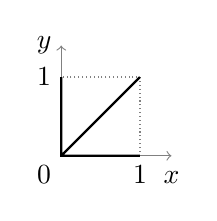
\begin{tikzpicture}
\draw[thin,gray,text=black,<->] (0,1.4) node[left] {$y$}
|- (1.4,0) node[below] {$x\vphantom{1}$};
\draw[densely dotted,gray] (1,0) |- (0,1);
\draw[thick] (0,1) node[left] {$1$} 
-- (0,0) node[below left] {$0$} 
-- (1,0) node[below] {$1$}
(0,0) -- (1,1);
\end{tikzpicture}

\caption{\label{fig:thick-counterexample}Thickness counterexample graph}
\end{figure}


$\Gamma$ is $\beta$-thick because $\rsupfun{\Gamma}\{0\}=[0;1]$.

To prove that $\Gamma$ is not $\alpha$-thick it's enough to prove
that every set $A$ such that $A\times A\subseteq\Gamma$ is finite.

Suppose for the contrary that $A$ is infinite. Then $A$ contains
more than one non-zero points $y$, $z$ ($y\ne z$). Without loss
of generality $y<z$. So we have that $(y;z)$ is not of the form
$(y;y)$ nor $(0;y)$ nor $(y;0)$. Therefore $A\times A$ isn't a
subset of $\Gamma$.
\end{proof}

\section{Totally bounded endoreloids}

The below is a straightforward generalization of the customary definition
of totally bounded sets on uniform spaces (it's proved below that
for uniform spaces the below definitions are equivalent).
\begin{defn}
\index{alpha
-totally bounded@$\alpha$-totally bounded}An endoreloid $f$ is \emph{$\alpha$-totally bounded} ($\totBound_{\alpha}(f)$)
if every~$E\in\up f$ is $\alpha$-thick.
\end{defn}

\begin{defn}
\index{beta
-totally bounded@$\beta$-totally bounded}An endoreloid $f$ is \emph{$\beta$-totally bounded} ($\totBound_{\beta}(f)$)
if every~$E\in\up f$ is $\beta$-thick.\end{defn}
\begin{rem}
We could rewrite the above definitions in a more algebraic way like
$\up f\subseteq\thick_{\alpha}$ (with $\thick_{\alpha}$ would be
defined as a set rather than as a predicate), but we don't really
need this simplification.\end{rem}
\begin{prop}
If an endoreloid is $\alpha$-totally bounded then it is $\beta$-totally
bounded.\end{prop}
\begin{proof}
Because $\thick_{\alpha}(E)\Rightarrow\thick_{\beta}(E)$.\end{proof}
\begin{prop}
If an endoreloid $f$ is reflexive and $\Ob f$ is finite then $f$
is both $\alpha$-totally bounded and $\beta$-totally bounded.\end{prop}
\begin{proof}
It enough to prove that $f$ is $\alpha$-totally bounded. Really,
every $E\in\up f$ is reflexive. Thus $\{x\}\times\{x\}\subseteq\GR E$
for $x\in\Ob f$ and thus $\setcond{\{x\}}{x\in\Ob f}$ is a sought
for finite cover of $\Ob f$.\end{proof}
\begin{obvious}
~
\begin{itemize}
\item A principal endoreloid induced by a $\mathbf{Rel}$-morphism $E$ is
$\alpha$-totally bounded iff $E$ is $\alpha$-thick.
\item A principal endoreloid induced by a $\mathbf{Rel}$-morphism $E$ is
$\beta$-totally bounded iff $E$ is $\beta$-thick.
\end{itemize}
\end{obvious}
\begin{example}
There is a $\beta$-totally bounded endoreloid which is not $\alpha$-totally
bounded.\end{example}
\begin{proof}
It follows from the example above and properties of principal endoreloids.
\end{proof}

\section{Special case of uniform spaces}

Remember that \emph{uniform space} is essentially the same as symmetric,
reflexive and transitive endoreloid.
\begin{thm}
Let $f$ be such an endoreloid that $f\circ f^{-1}\sqsubseteq f$.
Then $f$ is $\alpha$-totally bounded iff it is $\beta$-totally
bounded.\end{thm}
\begin{proof}
~
\begin{description}
\item [{$\Rightarrow$}] Proved above.
\item [{$\Leftarrow$}] For every $\epsilon\in\up f$ we have that $\rsupfun{\GR\epsilon}\{c_{0}\},\dots,\rsupfun{\GR\epsilon}\{c_{n}\}$
covers the space. $\rsupfun{\GR\epsilon}\{c_{i}\}\times\rsupfun{\GR\epsilon}\{c_{i}\}\subseteq\GR(\epsilon\circ\epsilon^{-1})$
because for $x\in\rsupfun{\GR\epsilon}\{c_{i}\}$ (the same as $c_{i}\in\rsupfun{\GR\epsilon}\{x\}$)
we have 
\[
\rsupfun{\rsupfun{\GR\epsilon}\{c_{i}\}\times\rsupfun{\GR\epsilon}\{c_{i}\}}\{x\}=\rsupfun{\GR\epsilon}\{c_{i}\}\subseteq\rsupfun{\GR\epsilon}\rsupfun{\GR\epsilon^{-1}}\{x\}=\rsupfun{\GR(\epsilon\circ\epsilon^{-1})}\{x\}.
\]
For every $\epsilon'\in\up f$ exists $\epsilon\in\up f$ such that
$\epsilon\circ\epsilon^{-1}\sqsubseteq\epsilon'$ because $f\circ f^{-1}\sqsubseteq f$.
Thus for every $\epsilon'$ we have $\rsupfun{\GR\epsilon}\{c_{i}\}\times\rsupfun{\GR\epsilon}\{c_{i}\}\subseteq\GR\epsilon'$
and so $\rsupfun{\GR\epsilon}\{c_{0}\},\dots,\rsupfun{\GR\epsilon}\{c_{n}\}$
is a sought for finite cover.
\end{description}
\end{proof}
\begin{cor}
A uniform space is $\alpha$-totally bounded iff it is $\beta$-totally
bounded.\end{cor}
\begin{proof}
From the theorem and the definition of uniform spaces.
\end{proof}
Thus we can say about just \emph{totally bounded} uniform spaces (without
specifying whether it is $\alpha$ or $\beta$).


\section{Relationships with other properties}
\begin{thm}
Let $\mu$ and $\nu$ be endoreloids. Let $f$ be a principal $\continuous'(\mu;\nu)$
continuous, monovalued, surjective reloid. Then if $\mu$ is $\beta$-totally
bounded then $\nu$ is also $\beta$-totally bounded.\end{thm}
\begin{proof}
Let $\varphi$ be the monovalued, surjective function, which induces
the reloid~$f$.

We have $\mu\sqsubseteq f^{-1}\circ\nu\circ f$.

Let $F\in\up\nu$. Then there exists $E\in\up\mu$ such that $E\subseteq\varphi^{-1}\circ F\circ\varphi$.

Since $\mu$ is $\beta$-totally bounded, there exists a finite typed
subset $A$ of $\Ob\mu$ such that $\rsupfun{\GR E}A=\Ob\mu$.

We claim $\rsupfun{\GR F}\rsupfun{\varphi}A=\Ob\nu$.

Indeed let $y\in\Ob\nu$ be an arbitrary point. Since $\varphi$ is
surjective, there exists $x\in\Ob\mu$ such that $\varphi x=y$. Since
$\rsupfun{\GR E}A=\Ob\mu$ there exists $a\in A$ such that $a\mathrel{(\GR E)}x$
and thus $a\mathrel{(\varphi^{-1}\circ F\circ\varphi)}x$. So $(\varphi a;y)=(\varphi a;\varphi x)\in\GR F$.
Therefore $y\in\rsupfun{\GR F}\rsupfun{\varphi}A$.\end{proof}
\begin{thm}
Let $\mu$ and $\nu$ be endoreloids. Let $f$ be a principal $\continuous''(\mu;\nu)$
continuous, surjective reloid. Then if $\mu$ is $\alpha$-totally
bounded then $\nu$ is also $\alpha$-totally bounded.\end{thm}
\begin{proof}
Let $\varphi$ be the surjective binary relation which induces the
reloid $f$.

We have $f\circ\mu\circ f^{-1}\sqsubseteq\nu$.

Let $F\in\up\nu$. Then there exists $E\in\up\mu$ such that $\varphi\circ E\circ\varphi^{-1}\subseteq F$.

There exists a finite cover $S$ of $\Ob\mu$ such that $\bigcup\setcond{A\times A}{A\in S}\subseteq\GR E$.

Thus $\varphi\circ\left(\bigcup\setcond{A\times A}{A\in S}\right)\circ\varphi^{-1}\subseteq\GR F$
that is $\bigcup\setcond{\rsupfun{\varphi}A\times\rsupfun{\varphi}A}{A\in S}\subseteq\GR F$.

It remains to prove that $\setcond{\rsupfun{\varphi}A}{A\in S}$ is
a cover of $\Ob\nu$. It is true because $\varphi$ is a surjection
and $S$ is a cover of $\Ob\mu$.
\end{proof}
A stronger statement (principality requirement removed):
\begin{conjecture}
The image of a uniformly continuous entirely defined monovalued surjective
reloid from a ($\alpha$-, $\beta$-)totally bounded endoreloid is
also ($\alpha$-, $\beta$-)totally bounded.
\end{conjecture}
Can we remove the requirement to be entirely defined from the above
conjecture?
\begin{question}
Under which conditions it's true that join of ($\alpha$-, $\beta$-)
totally bounded reloids is also totally bounded?
\end{question}

\section{Additional predicates}

We may consider also the following predicates expressing different
kinds of what is intuitively is understood as boundness. Their usefulness
is unclear, but I present them for completeness.
\begin{itemize}
\item $\totBound_{\alpha}(f)$
\item $\totBound_{\beta}(f)$
\item $\exists n\in\mathbb{N}\forall E\in\up f:\thick_{\alpha}(E^{n})$
\item $\exists n\in\mathbb{N}\forall E\in\up f:\thick_{\beta}(E^{n})$
\item $\exists n\in\mathbb{N}\forall E\in\up f:\thick_{\alpha}(E^{0}\sqcup\ldots\sqcup E^{n})$
\item $\exists n\in\mathbb{N}\forall E\in\up f:\thick_{\beta}(E^{0}\sqcup\ldots\sqcup E^{n})$
\item $\exists n\in\mathbb{N}:\totBound_{\alpha}(f^{n})$
\item $\exists n\in\mathbb{N}:\totBound_{\beta}(f^{n})$
\item $\exists n\in\mathbb{N}:\totBound_{\alpha}(f^{0}\sqcup\ldots\sqcup f^{n})$
\item $\exists n\in\mathbb{N}:\totBound_{\beta}(f^{0}\sqcup\ldots\sqcup f^{n})$
\item $\totBound_{\alpha}(S(f))$
\item $\totBound_{\beta}(S(f))$
\end{itemize}
Some of the above defined predicates are equivalent:
\begin{prop}
~
\begin{itemize}
\item $\exists n\in\mathbb{N}\forall E\in\up f:\thick_{\alpha}(E^{n})\Leftrightarrow\exists n\in\mathbb{N}:\totBound_{\alpha}(f^{n})$.
\item $\exists n\in\mathbb{N}\forall E\in\up f:\thick_{\beta}(E^{n})\Leftrightarrow\exists n\in\mathbb{N}:\totBound_{\beta}(f^{n})$.
\end{itemize}
\end{prop}
\begin{proof}
Because for every $E\in\up f$ some $F\in\up f^{n}$ is a subset of $E^{n}$, we have
\[\forall E\in\up f:\thick_{\alpha}(E^{n})\Leftrightarrow\forall F\in\up f^n:\thick_{\alpha}(F)\]
and likewise for $\thick_{\beta}$.\end{proof}
\begin{prop}
~
\begin{itemize}
\item $\exists n\in\mathbb{N}\forall E\in\up f:\thick_{\alpha}(E^{0}\sqcup\ldots\sqcup E^{n})\Leftrightarrow\exists n\in\mathbb{N}:\totBound_{\alpha}(f^{0}\sqcup\ldots\sqcup f^{n})$
\item $\exists n\in\mathbb{N}\forall E\in\up f:\thick_{\beta}(E^{0}\sqcup\ldots\sqcup E^{n})\Leftrightarrow\exists n\in\mathbb{N}:\totBound_{\beta}(f^{0}\sqcup\ldots\sqcup f^{n})$
\end{itemize}
\end{prop}
\begin{proof}
It's enough to prove
\begin{align}
\label{thk-1}&\forall E\in\up f\exists F\in\up(f^0\sqcup\dots\sqcup f^n):F\sqsubseteq E^{0}\sqcup\ldots\sqcup E^{n} \text{ and}\\
\label{thk-2}&\forall F\in\up(f^0\sqcup\dots\sqcup f^n)\exists E\in\up f:E^{0}\sqcup\ldots\sqcup E^{n}\sqsubseteq F.
\end{align}

For the formula~\eqref{thk-1} take $F=E^0\sqcup\dots\sqcup E^n$.

Let's prove~\eqref{thk-2}. Let $F\in\up(f^0\sqcup\dots\sqcup f^n)$. Take
$E_i\in\up f$ for $i=0,\dots,n$ such that $E_i^i\sqsubseteq F$ (exercise~\ref{rld-fn} and properties of generalized filter bases) and then $E=E_{0}\sqcap\dots\sqcap E_{n}\in\up f$. We have
$E^{0}\sqcup\ldots\sqcup E^{n}\sqsubseteq F$.
\end{proof}
\begin{prop}
All predicates in the above list are pairwise equivalent in the case
if $f$ is a uniform space.\end{prop}
\begin{proof}
Because $f\circ f=f$.\end{proof}

